\begin{pastexam}[label={px:ncku-114-ee-ds-02}]{成大電機所 114 學年度 單選題第 2 題}
（單選；每題 5 分，答錯倒扣 2 分）

Given that the post-order traversal of a binary tree is ``E F B C D A'' and the in-order
traversal of the same tree is ``E F A C B D'', please provide the resulting pre-order traversal
of the tree.
\begin{enumerate}[label=\alph*)]
\item A F E D C B
\item A E F D C B
\item A F E C D B
\item A F E B C D
\item None of the above.
\end{enumerate}
\end{pastexam}

\begin{pastsoln}
答案是 a) A F E D C B。

後序的最後一個是根，在中序裡找到根，左邊是左子樹、右邊是右子樹（資結書第~7.4~節）：
\begin{center}
\begin{tabular}{llcll}
\toprule
子樹的後序 & 子樹的中序 & 根 & 左子樹（中序） & 右子樹（中序） \\
\midrule
EFBCDA & EF\,$|$\,A\,$|$\,CBD & A & EF & CBD \\
EF & E\,$|$\,F\,$|$ & F & E & 空 \\
BCD & CB\,$|$\,D\,$|$ & D & CB & 空 \\
BC & $|$\,C\,$|$\,B & C & 空 & B \\
\bottomrule
\end{tabular}
\qquad
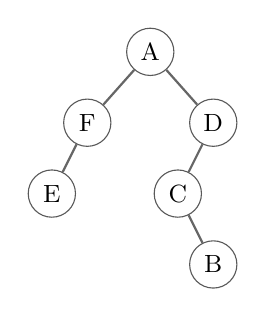
\begin{tikzpicture}[baseline=(r.center),
    btn/.style={circle, draw=black!65, line width=0.4pt, minimum size=6mm, inner sep=0pt, font=\small},
    level distance=9mm, edge from parent/.style={draw=black!60, thick},
    level 1/.style={sibling distance=16mm}, level 2/.style={sibling distance=9mm}]
\node[btn] (r) {A}
    child {node[btn] {F} child {node[btn] {E}} child[missing]}
    child {node[btn] {D} child {node[btn] {C} child[missing] child {node[btn] {B}}} child[missing]};
\end{tikzpicture}
\end{center}
左子樹有 $2$ 個節點，所以後序的前 $2$ 個（E F）是左子樹、接著 $3$ 個（B C D）是右子樹。
前序（根、左、右）：A，左子樹 F E，右子樹 D C B，得 \textbf{A F E D C B}。 驗算：這棵樹的後序是
E F B C D A、中序是 E F A C B D，和題目一致。

其他選項：b) 把左子樹寫成 E F（那是中序或後序的順序，不是前序）；c) 把 C、D 對調，D 是右子樹的
根要先出現；d) 右子樹寫成 B C D，是後序的順序。
\end{pastsoln}
